\documentclass[mathserif]{beamer}
\usetheme{madrid}
\title{Three Curves}
\author{20513322}
\date{May 14 2023}
\begin{document}
\begin{frame}
\maketitle
\end{frame}
\begin{frame}
\frametitle{Outline}
\tableofcontents
\end{frame}
\section{Frame3}
\begin{frame}\label{3}
\frametitle{Three Curves}
\begin{columns}
\column{0.5\textwidth}<1->
$$
\left\{
\begin{array}{lll}
f(x)&=&e^{1-x^2}\\
g(x)&=&2xe^{x^2-1}\\
h(x)&=&-x\sin x+3\ln(x+1)
\end{array}
\right.
$$
\column{0.5\textwidth}<2->
\begin{figure}
\centering
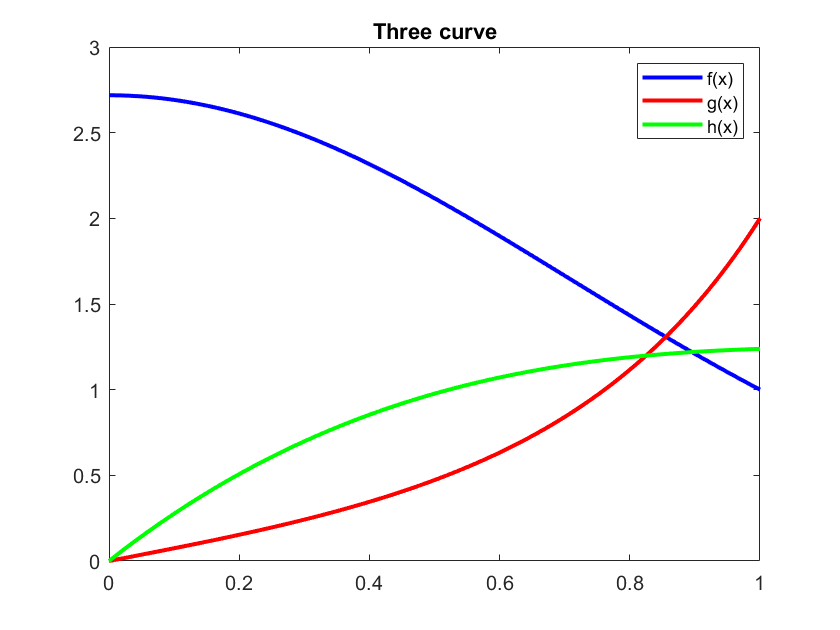
\includegraphics[scale=0.3]{Q2a}
\end{figure}
\end{columns}
\end{frame}
\section{Frame4}
\begin{frame}
\frametitle{Observation}
\begin{block}{Derivative}
\begin{itemize}
\item First order derivative $f(x)$ is \textbf{negative} on interval $[0, 1]$.
\item First order derivatives of $g(x)$ and $h(x)$ are \textbf{positive} on interval $[0, 1]$.
\begin{itemize}
\item[-] Second order derivative of $g(x)$ is \underline{positive} on interval $[0, 1]$.
\item[-] Second order derivative of $g(x)$ is \underline{negative} on interval $[0, 1]$.
\end{itemize}
\end{itemize}
\end{block}
\hyperlink{3}{\beamerbutton{CLICK HERE}}for three curves
\end{frame}
\begin{frame}[fragile]
\begin{verbatim}
$$
\left\{
\begin{array}{lll}
f(x)&=&e^{1-x^2}\\
g(x)&=&2xe^{x^2-1}\\
h(x)&=&-x\sin x+3\ln(x+1)
\end{array}
\right.
$$
\end{verbatim}
\end{frame}
\begin{frame}
\begin{columns}
\column{0.5\textwidth}
$$
\left\{
\begin{array}{lll}
f(x)&=&e^{1-x^2}\\
g(x)&=&2xe^{x^2-1}\\
h(x)&=&-x\sin x+3\ln(x+1)
\end{array}
\right.
$$
\column{0.5\textwidth}
$$
\left\{
\begin{array}{lll}
f(x)&=&e^{1-x^2}\\
g(x)&=&2xe^{x^2-1}\\
h(x)&=&-x\sin x+3\ln(x+1)
\end{array}
\right.
$$
\end{columns}
\end{frame}
\end{document}
